\section{The Standard Model}
Everything this thesis is built on has its roots in the Standard Model (SM). The Standard Model of particle physics addresses the question \emph{What is matter made of?} on the smallest possible scale. It links the fundamental constituents of the universe together along with the forces that bind them, in order to describe ad predict the laws of nature. The Standard Model is formulated as a quantum field theory, where the fundamental particles are spin-1/2 fermions which interact with one another through the exchange of spin-1 gauge bosons. These interactions come in three forms, mediated by three different types of gauge bosons: The electromagnetic force, mediated through photons; the weak force, mediated through W and Z bosons; and the strong force, mediated by gluons. How the fundamental particles interact also defines which properties they exhibit. In addition, the Standard Model includes a field very different from the others, the Higgs field. The Higgs field interacts both fermions and bosons and is what gives all particles their mass.\newline
One thing the Standard Model fails to incorporate is the force of gravity. This shortcoming is one of the main motivations for looking for alternative models beyond the Standard Model (BSM), which is the main topic of this thesis.

\subsection{Fundamental particles: Quarks and leptons}
It appears that all matter in the universe can be described by a very small collection of fundamental particles, six leptons and six quarks. These are collectively called fermions and are, as far as we can tell, truly elementary (not composed of any other particles).
Leptons are particles with integer or zero electric charge, defined in units of electron charge. They come in three flavors, or generations, and their mass increases with generation. Each generation of leptons consists of two particles: one charged lepton and one neutrally charged particle denoted \emph{neutrino ($\nu$)}. The three generations can be arranged in a doublet structure, and are as follows
\begin{equation}
\label{eqn:lepton_flavor_doublets}
\begin{pmatrix} \nu_e      \\ e      \end{pmatrix} \qquad
\begin{pmatrix} \nu_{\mu}  \\ \mu    \end{pmatrix} \qquad
\begin{pmatrix} \nu_{\tau} \\ \tau   \end{pmatrix}
\end{equation}
The charged leptons can be positively or negatively charged, defined in units of electron charge $e$. By convention the leptons of matter are negatively charged, $e^{-}$, $\mu^{-}$, and $\tau^{-}$,  whereas the positively charged leptons,  $e^{+}$, $\mu^{+}$, and $\tau^{+}$ are considered their anti-particles.
% Each lepton generation is assigned its own quantum number $L$ which must be conserved after any process.
A summary of the lepton properties is listed in Table~\ref{table:theory:lepprop}.
\begin{table}[h!]
\begin{center}
\begin{tabular}{|c|c|c|}% c c c|}
\hline
Lepton        & Mass           & Charge \\%& $L_{e}$ & $L_{\mu}$ & $L_{\tau}$ \\
\hline
$e^{-}$      & $0.5 \mbox{ MeV}$      & $e$ \\%& 1       & 0         & 0 \\
$\mu^{-}$    & $106 \mbox{ MeV}$      & $e$ \\%& 0       & 1         & 0 \\
$\tau^{-}$   & $1777 \mbox{ MeV}$     & $e$ \\%& 0       & 0         & 1 \\
\hline                                      
$\nu_{e}$    & $< 3 \mbox{ eV}$       & $0$ \\%   & 1       & 0         & 0 \\
$\nu_{\mu}$  & $< 0.19 \mbox{ MeV}$   & $0$ \\%   & 0       & 1         & 0 \\
$\nu_{\tau}$ & $< 18.2 \mbox{ MeV}$   & $0$  \\%   & 0       & 0         & 1 \\
\hline
\end{tabular}
\end{center}
\caption{Lepton Properties}
\label{table:theory:lepprop}
\end{table}
Leptons interact with one another through the \emph{electromagnetic and weak force}, which will be explained in more detailed in Section~\ref{sec:theory:ew}.\newline
The other six fundamental particles of matter are the \emph{quarks}. They are distinguished from the leptons in that they interact with one another through the \emph{strong force}, described in Section~\ref{sec:theory:qcd}. This force binds the quarks together to form baryons (like protons and neutrons) or mesons (like pions), and in addition, keeps the quarks from being observed as free particles such that they are only visible through their baryon/meson bound states. Also organized in three generations, the six quarks are called \textit{up}, \textit{down}, \textit{charm}, \textit{strange}, \textit{top} and \textit{bottom}, and are organized in flavor doublets as follow
\begin{equation}
\label{eqn:quark_flavor_doublets}
\begin{pmatrix} u \\ d \end{pmatrix} \qquad
\begin{pmatrix} c \\ s \end{pmatrix} \qquad
\begin{pmatrix} t \\ b \end{pmatrix}
\end{equation}
Each quark comes with a fractional charge of $\frac{2}{3}$ (u, c and t) and $-\frac{1}{3}$ (d, s and b) of one electron charge. As with the leptons, there are also distinct particles of opposite charge, anti-quarks. As mentioned above, quarks can interact with one another through the strong force. However, they also interact through the weak and electromagnetic forces.
Some of the quark properties are listed in Table~\ref{table:theory:quarkprop}.
\begin{table}
\begin{center}
\begin{tabular}{|c|c|c|}%c|}
\hline
Quark & Mass & Charge \\% & Properties \\
\hline
u & $1-5 \mbox{ MeV}$         & $\phantom{-}\frac{2}{3} e$  \\%& $I_{z} = \frac{1}{2}$ \\
d & $3-9 \mbox{ MeV}$         & $-\frac{1}{3} e$            \\%& $I_{z} = -\frac{1}{2}$ \\
c & $1.15-1.35 \mbox{ GeV}$   & $\phantom{-}\frac{2}{3} e$  \\%& Charm = +1 \\
s & $75-170 \mbox{ MeV}$      & $-\frac{1}{3}e$             \\%& Strangeness = -1 \\
t & $172.4\pm 0.1 \mbox{ GeV}$ & $\phantom{-}\frac{2}{3} e$  \\%& Top = +1 \\
b & $4.0-4.4 \mbox{ GeV}$     & $-\frac{1}{3} e$            \\%& Bottom = -1 \\
\hline
\end{tabular}
\end{center}
\caption{Quark Properties}
\label{table:theory:quarkprop}
\end{table}
These 12 fermions, together with their corresponding anti-particles, represent the fundamental particles of the universe and constitute all matter around us. There are four fundamental forces that we know of: gravity, electromagnetism, the weak force and the strong force. Gravity is extremely weak compared to the other forces and we currently lack a quantum field theory of its interaction, therefore it is typically ignored in high energy physics experiments. 
All particles that are electrically charged, the charged leptons ($e$, $\mu$ and $\tau$) and all of the quarks, interact through the electromagnetic force. These interactions are governed by the laws of Quantum Electrodynamics (QED), and are mediated through the massless and electrically neutral spin-1 photons. All of the fermions, including the electrically neutral neutrinos, feel the weak force and undergo weak interactions. The weak force is mediated through vector bosons ($PW^+$, $PW^-$ and $Z^0$), which are heavy charged particles with a spin of 1. Finally, there is the strong force, mediated by the massless and electrically neutral spin-1 gluon. Only quarks interact via the strong force, and it is that interaction that makes the quarks so fundamentally different from electrons and neutrinos. The strong force keeps us from observing quarks as free particles, and keeps them in bound states referred to as \emph{hadrons}. Their interaction is governed by the laws of Quantum Chromodynamics (QCD). All of these interactions can be represented in one common gauge theory, the Standard Model.

\subsection{The Standard Model Lagrangian}
\label{sec:theory:gauge}
The Standard Model is a quantum gauge field theory in which each particle is described as a dynamical field with a value at each space-time coordinate. These fields are governed by a Lagrangian density function, the Standard Model. For instance, the Lagrangian density of a free fermion, one not interacting with any other fields, is
\begin{equation}
  \mathcal{L} = \bar{\Psi}(x^{\mu})(i\lambda^{\mu}\partial_{\mu}-m)\Psi(x^{\mu})
\end{equation}
where $\Psi(x^{\mu})$ represents any spin-1/2 fermion field, also called \emph{Dirac field}, as a function of space-time; $\bar{\Psi}=\Psi^{\dagger}\gamma_0$, where $\gamma^0$ is one of the gamma matrices $\gamma^{\mu}$, which is included in order to make $\Psi^{\dagger}\Psi$ invariant under Lorentz transformation; and $m$ is the mass of the fermion in question. Any interaction between the fundamental particles due to the fundamental forces, can be described as variations in the Lagrangian of quantum fields and are represented as additional terms in the equation above.\newline
Being a gauge theory, the Standard Model has the property of gauge invariance, meaning that measurable quantities stay the same despite the fields themselves changing. If observables stay the same after a field transformation, there is a symmetry in the system. The symmetries of the Standard Model arise due to the fact that fermions of a given type are indistinguishable from one another. These symmetries result in the presence of \emph{force mediators}, which arise as a representation of infinitesimal generators of some symmetry group.
 %The spin-1/2 fermion fields are arranged in \emph{Weyl spinors}, listen in Equation~\ref{eqn:lepton_flavor_doublets} and~\ref{eqn:quark_flavor_doublets}, which transform differently depending on their quantum numbers. 
The fermion fields can be arranged as particle multiplets where one transforms into the other under a symmetry transformation. A symmetry transformation produce rotations between the particles of a given multiplet, but never to a field outside of that group. The symmetry group of the Standard Model is the direct product
\begin{equation}
  SU(3)_C \otimes SU (2)_L \otimes U(1)_Y.
\end{equation}
$SU(3)_C$ is the color $C$ symmetry allowing the rotation of quarks, arranged in color multiplets, into one another, corresponding to interactions produced by the strong force. The colors are denoted as red, green and blue. $SU (2)_L \otimes U(1)_Y$ represent the electroweak force with weak left-handed isospin $L$ and weak hypercharge $Y$ symmetries, acting on $L$ and $Y$ multiplets, respectively. %These forces, together with their conserved charges, will be clarified in the sections below.
The particle multiplets of the Standard Model can then be written as $\mathcal{G}_{SM} \ni x=(C,L)_{(Y)}$ (here for the 1st generation only) and are:
\begin{alignat*}{3}
Q &= (3,2)_{(1/3)} &&=
  \begin{pmatrix} 
    u_r & u_g & u_b \\
    d_r & d_g & d_b
    \end{pmatrix} \quad  &&\sim \textrm{quark multiplet} \\[1pt]
L &= (1,2)_{(-1)} &&= \begin{pmatrix} \nu_e & e \end{pmatrix} \quad &&\sim \textrm{leptonic doublet} \\[1pt]
u^c &= (\bar{3},1)_{(-4/3)} &&= \begin{pmatrix} u_{\bar{r}}^c & u_{\bar{g}}^c & u_{\bar{b}}^c\end{pmatrix} \quad &&\sim \textrm{anti-up quarks} \\[1pt]
d^c &= (\bar{3},1)_{(2/3)}  &&= \begin{pmatrix} d_{\bar{r}}^c & d_{\bar{g}}^c & d_{\bar{b}}^c\end{pmatrix} \quad &&\sim \textrm{anti-down quarks} \\[1pt]
e^c &= (1,1)_{(2)}          && \quad &&\sim \textrm{positron} \\
\end{alignat*}
The anti-neutrino is not included here because it is a SM \emph{singlet} and does not transform under the SM group $\mathcal{G}_{SM}$, but it could be written as $\nu^c=(1,1)_(0)$. The positron $e^c$, on the other hand, \emph{is} included as its hypercharge is non-zero and it therefore undergoes $U(1)_Y$ interactions. These five multiplets exist for each of the tree generations.\newline
The numbers representing each multiplet correspond to which representation it belongs to. For instance, we see that the quark multiplet transforms as a triplet under $SU(3)_C$, a doublet under $SU(2)_L$ and has a non-zero hypercharge, corresponding to a non-trivial representation under $U(1)_Y$. That corresponds to saying that quarks interact through all of the three fundamental interactions. From that notation, it is also clear that leptons do not carry color charge and will only interact via the electroweak interactions.\newline
From the multiplets above, we see that $u^c$ and $d^c$ transform as singlets under $SU(2)_L$, meaning they do not interact. This, however, does not mean they do not feel the electroweak force. The electroweak gauge bosons \PW and \PZ are not directly part of $SU(2)_L$, rather, they are a linear combination of $SU(2)_L$ and $U(1)_Y$ and anything with a non-zero weak hypercharge $Y$ will interact with them. This is also true for the photon, which also is a linear combination of $SU(2)_L$ and $U(1)_Y$.\newline
These interactions; the strong, weak and electromagnetic, will be explained in more detail in the following sections.

\subsubsection{The Quantum Chromodynamics sector}
\label{sec:theory:qcd}
The group $SU(3)_C$ describe the strong interaction mediated by gluons, and is described by the quantum gauge theory Quantum Chromodynamics (QCD). The group is generated by 8 linearly independent matrices $T^a=\frac{\lambda^a}{2}$, where $\lambda^a$ are the Gell-Mann matrices~\cite{PhysRev.125.1067}. The generator matrices do not commute with one another, but rather satisfy the commutation relation $[\lambda^i/2,\lambda^j/2]=i f^{ijk} \lambda_k/2$. This property makes $SU(3)_C$ group \emph{non-Abelian}, which consequently results in the gluons themselves being charged and display self-interactions. Gluons are charged with one unit of color and one unit of anti-color. Quarks, the only fundamental particles interacting with the strong force, are arranged in the simplest representation of $SU(3)$ and come with one unit of color or anti-color. \newline
The generators are collectively referred to as the \emph{group representation} of $SU(3)_C$, because any group element can be can be written as $e^{-i\theta^a g_a}$, where $a$ runs from 1 to 8, $\theta^a$ are real numbers and $g_a$ represent one of the eight linearly independent $\lambda/2$ matrices. That means that, given one representation, one can always find another one through any local gauge transformation that leaves the commutator unchanged.  
In this case, the group elements are the quark fields, and a local gauge transformation of fields become
\begin{equation}
  \Psi(x^{\mu}) \rightarrow e^{ -i g_s \theta^a(x^{\mu}) T^a}\Psi(x^{\mu})
\end{equation}
where $g_s$ is the strong coupling, $\theta^a(x^{\mu})$ some arbitrary function and $a$ runs over the eight generators of the group. In order to keep the QCD Lagrangian invariant under such a transformation, an additional term must be added, replacing the partial derivative $\partial_{\mu}$ with
\begin{equation}
  D_\mu=\partial_\mu + ig_s \mathcal{A}_{\mu}^a T^a,
\end{equation}
where we now have introduced a tensor $\mathcal{A}_{\mu}^a$ that represents the 8 gluon fields.
The QCD Lagrangian then becomes
\begin{equation}
  \label{eq:theory:qcdl}
   \mathcal{L}_{QCD} =-\frac{1}{4}{\cal F}_{a}^{\mu\nu}{\cal F}^{a}_{\mu\nu}+\bar{\Psi}(x^{\mu})(i\lambda^{\mu}D_{\mu}-m)\Psi(x^{\mu}),
\end{equation}
where $F_{\mu\nu}^a$ is the gauge field of the group, the gluon field tensor 
\begin{equation}
F_{\mu\nu}^a=\partial_{\mu} \mathcal{A}_{\nu}^a-\partial_{\nu} \mathcal{A}_{\mu}^a+g_s f^{abc}\mathcal{A}_{\mu}^b\mathcal{A}_{\nu}^c.
\end{equation}
The first term in Equation~\ref{eq:theory:qcdl} represents the quark-gluon interaction, leading to vertices like the one on the right in Figure~\ref{fig:theory:qcdint}. The second, the gluon field kinetic term, pick up the \emph{structure constant} $f^{abc}$ due to the commutation relation of the $\lambda$ matrices. This term creates self-interactions between the gluon fields, like the two shown on the right in Figure~\ref{fig:theory:qcdint}.
\begin{figure}[h!]
\centering
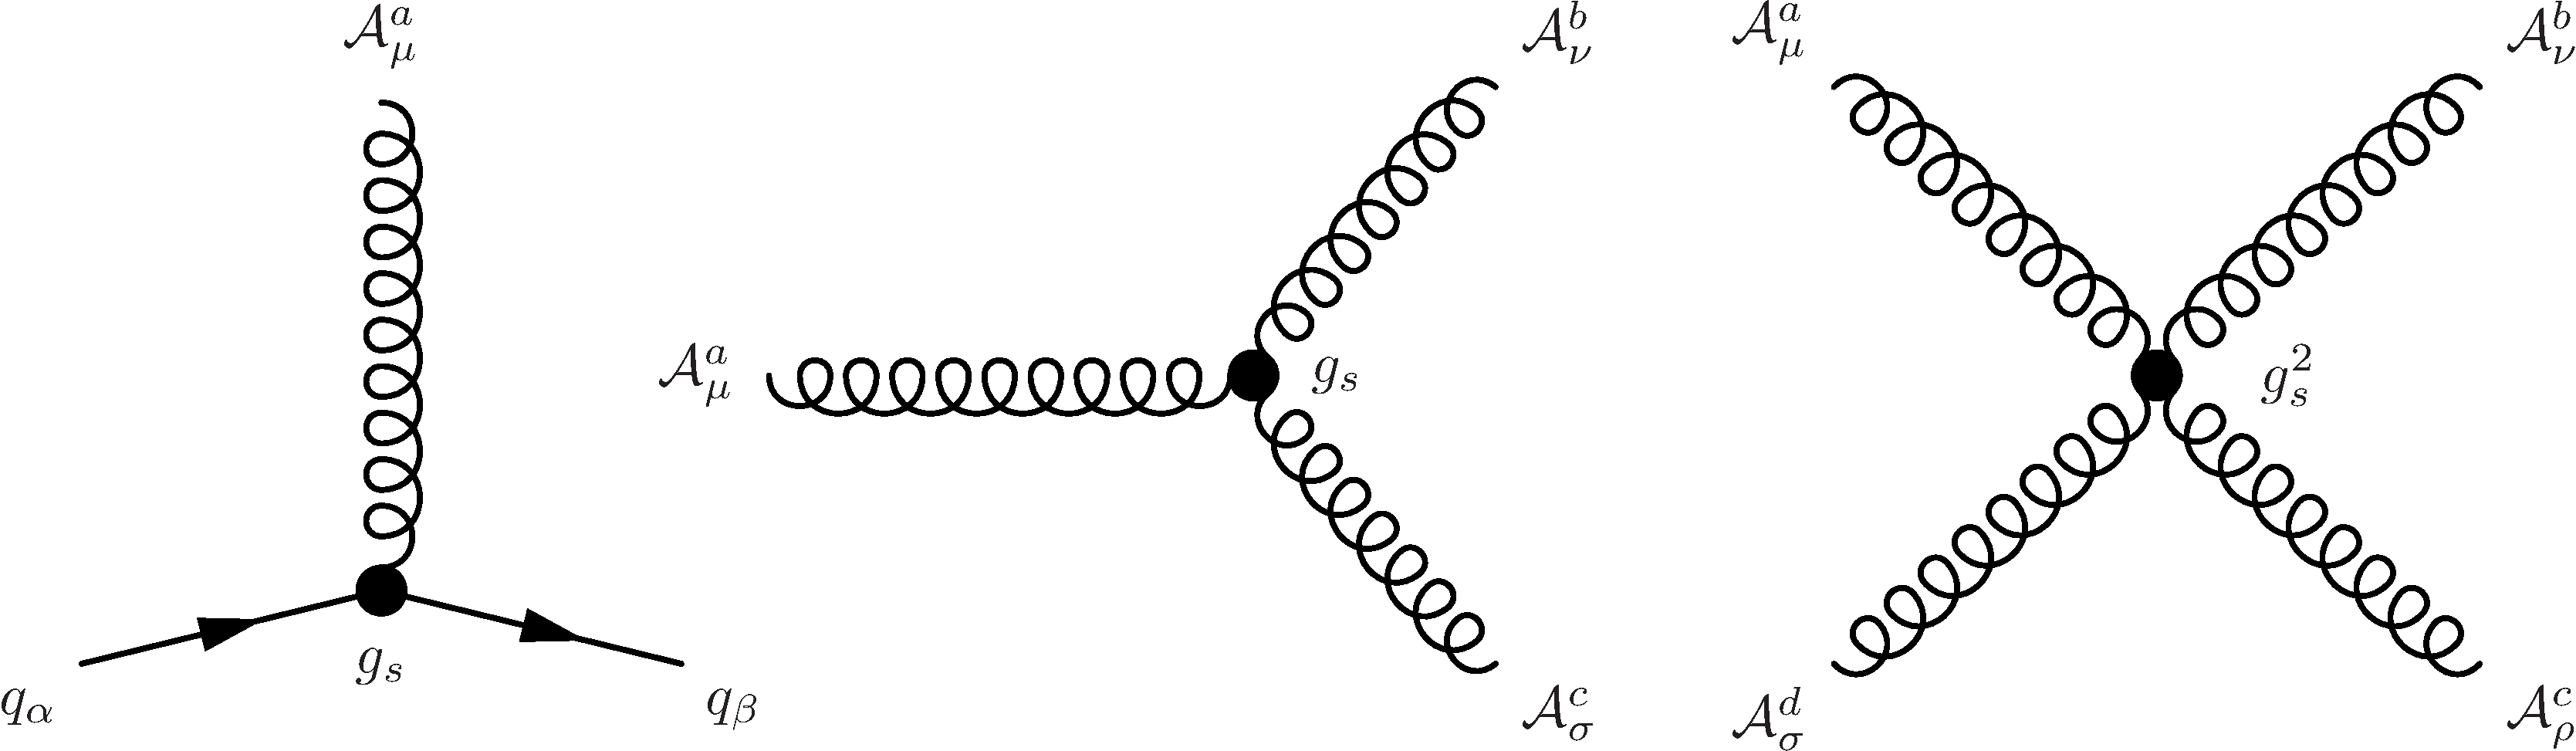
\includegraphics[width=0.79\textwidth]{figures/theory/QCD_vtx.pdf}
\caption{The QCD interaction vertices: Quark interaction with the gluon field (left), and three- (middle) and four-gluon (right) self-interaction vertices.}
\label{fig:theory:qcdint}
\end{figure}
These self-interactions have severe consequences: any bare color charge, like a quark, will be surrounded by a sea of virtual gluons and quarks that share the same color. When probing the quark color at higher and higher energies, corresponding to shorter and shorter distances, the color charge decreases until only the bare charge is visible. There, the quarks are essentially free and can be observed as distinguishable particles. This property is referred to as \emph{asymptotic freedom}. For the same reasons, when going further and further away from a bare color charge, the sea of charges surrounding it makes the observed charge increase. That results in a strong attractive force between color charges at large distances, where the potential energy between the two grows linearly with the distance between them as
\begin{equation}
  V(r)=-\frac{4\alpha_s}{3r}+kr,
\end{equation} 
where $r$ is the distance between the quarks and $\alpha_s$ is the coupling strength of QCD, describing how the observed charge between two quarks increases depending on the distance between them. When the distance between the quarks grows very large, this potential energy is enough to create real quark-antiquark pairs from the vacuum in order to reduce the potential energy, a process called \emph{fragmentation}. Whenever one tries to separate quarks form one another they will fragment, which consequently means that quarks are never observed on their own. Rather, they form colorless (uncharged under the color charge) bound states of mesons or baryons (collectively called hadrons), a property called \emph{color confinement}. The energy for which the confinement into hadrons occurs, also called \emph{hadronization}, is defined through experimental measurement and found to be $\Lambda_{QCD}=100-500 \MeV$ (around the mass of the lightest hadrons). The effective charge between the quarks, $\alpha_S$, changes as a function of energy as
 \begin{equation}
   \alpha_S(Q)=-\frac{6\pi}{33-2n_f}\ln(Q/\Lambda_{QCD})
 \end{equation}
where $Q$ is the energy of the probe used to measure the charge and $n_f$ is the number of quark flavors (u, d, c, s, b, t) at that energy. $\alpha_S$ is around 0.1 for energies between 100-1000 \GeV.

\subsection{The electroweak sector}
\label{sec:theaory:ew}
The electromagnetic and weak interactions arise from the breaking of $SU (2)_L \otimes U(1)_Y$ symmetry. The symmetry under $SU (2)_L$ is called weak left-handed isospin $L$, and the symmetry under $U(1)_Y$ is the weak hypercharge $Y$.
The name "left-handed" arise from the fact that \emph{parity} is violated in the electroweak interactions. All the fundamental fermions have a \emph{chirality}, defined as the projection of the particles spin along its direction of motion. From observations, the weak interactions is observed to only interact with fermions of left-handed chirality (vector minus axial coupling, V-A). The left-handed fermion fields are therefore in the simplest doublet representation of $SU(2)$ with weak isospin $I=1/2$, while the fermions of right-handed chirality are in the singlet representation with weak isospin $I=0$, meaning they do not interact with the gauge bosons of $SU (2)_L$. To obtain the correct chiral components $\Psi_L$ and $\Psi_R$,
The chirality of any fermion $\Psi$ can be defined through the operator $\gamma^5$, the product of the four Dirac matrices~\cite{Pauli:1936gd} $\gamma^5=i\gamma^1\gamma^2\gamma^3\gamma^4$, which has eigenvalues $\pm 1$. Any Dirac field can be projected into its chiral components $\Psi_L$ or $\Psi_R$ through the projection operation
\begin{equation}
  \Psi_L = \frac{1-\gamma^5}{2} \quad \textrm{and} \quad \Psi_R = \frac{1+\gamma^5}{2}.
  \end{equation}
The gauge field tensor of the group of $SU (2)_L$ symmetry (similar to the gluon tensor $\mathcal{A}_{\nu}^a$ we saw above) is $W_{\mu\nu}^a$, where $a$ runs over the 3 generators of the group. The conserved charge associated with the group is the \emph{third} component of weak isospin $I_3$, and all weak interactions must preserve $I_3$. The generators of the group are defined as $T_i=\frac{\sigma_i}{2}$, where $\sigma_i$ are the Pauli matrices~\cite{inbook}. The group is non-abelian and the generators follow the commutation relation $[\sigma_i/2,\sigma_j/2]=i \epsilon_{ijk} \sigma_k/2$, where $\epsilon_{ijk}$ is the Levi-Civita permutation symbol~\cite{Duplij2004}. This in turn implies self-interactions between the generators of the group, as was the case for $SU(3)_C$. The left-handed fermion fields are doublets under $SU (2)_L$, while the right-handed components transform as singlets and hence do not interact with the gauge field tensor. \newline
The latter group, $U(1)_Y$ of weak hypercharge $Y$, is abelian and hence display no self-interaction. The gauge field tensor $B_{\mu\nu}^a$ interacts with both left- and right-handed Dirac fields. As mentioned above, the photon, mediator of the electromagnetic force through electromagnetic charge, is a linear combination of $SU(2)_L$ and $U(1)_Y$. The electric charge is therefore defined through weak isospin and hypercharge as
\begin{equation}
  Q = I_3 + \frac{Y}{2}.
\end{equation}
Similar to the case for QCD, a local gauge transformation of $SU (2)_L \otimes U(1)_Y$ requires the addition of additional terms in the derivate in order to keep the Lagrangian invariant and the partial derivative $\partial_{\mu}$ is replaced by
\begin{align}
  D_\mu \Psi_L &=(\partial_{\mu} + ig_2 T_a W_{\mu}^a + ig_1 \frac{Y}{2} B_{\mu}^a)\Psi_L\\
  D_\mu \Psi_R &=(\partial_{\mu} + ig_1 \frac{Y}{2} B_{\mu}^a)\Psi_R.
\end{align}
The electroweak Lagrangian can be written as a sum of four terms
% \begin{equation}
%   \label{eq:theory:ewl}
%    \mathcal{L}_{EW} =-\frac{1}{4}{\cal W}_{a}^{\mu\nu}{\cal W}^{a}_{\mu\nu} - \frac{1}{4}{\cal B}^{\mu\nu}{\cal B}_{\mu\nu} +\bar{\Psi_L}(x^{\mu})(i\lambda^{\mu}D_{\mu}-m)\Psi(x^{\mu}),
% \end{equation}
\begin{equation}
  \label{eq:theory:ewl}
   \mathcal{L}_{EW} = \mathcal{L}_{gauge}+\mathcal{L}_{\phi}+\mathcal{L}_{f}+\mathcal{L}_{Yukawa}.
\end{equation}
The first term, $\mathcal{L}_{gauge}$, represent the kinetic field tensor and is
\begin{equation}
  \label{eq:theory:gauge}
   \mathcal{L}_{gauge} = -\frac{1}{4}{\cal W}_{a}^{\mu\nu}{\cal W}^{a}_{\mu\nu} - \frac{1}{4}{\cal B}^{\mu\nu}{\cal B}_{\mu\nu}
\end{equation}
where the gauge field tensors are
\begin{align}
W_{\mu\nu}^a &=\partial_{\mu} \mathcal{W}_{\nu}^a-\partial_{\nu} \mathcal{W}_{\mu}^a-g_2\epsilon^{ijk}{\cal W}^{j}_{\mu}{\cal W}^{k}_{\nu} \quad \textrm{, with   } i=1-3\\
B_{\mu\nu} &=\partial_{\mu} \mathcal{B}_{\nu}-\partial_{\nu} \mathcal{B}_{\mu}.
\end{align}
The non-abelian nature of $SU (2)_L$ lead to trilinear and quadrilinear couplings between the photon and vector bosons as illustrated in Figure~\ref 
\subsection{The Higgs Mechanism}

 
\clearpage

\section{Beyond Standard Model Physics}
Despite being an extremely successful and predictive theory, the Standard Model has its shortcomings. The most obvious one is its failure to successfully incorporate the gravitational force. Gravity is beautifully described in General Relativity as a classical theory: a force caused by the curvature of space-time in the presence of matter and energy. The theory does not utilize quantum fields and energy is not quantized.
The scales between the Standard model, a quantum field theory, and General Relativity are completely different: space-time is curved on astronomical scales, where the force of gravity is measurable, while quantum field theories deal with things on the smallest possible scales, where variations in space-time are essentially invisible. Hence, to the Standard Model, space-time is approximately flat and gravity does not exist. In order to have an elegant unified theory of all the forces, attempts has been made to have a quantum field theory of the gravitational force by extending the Standard Model particle family to incorporate a particle to mediate the gravitational force called the \emph{graviton}, a massless gauge boson of spin-2. The problem is that gravity is universally attractive, meaning nothing "cancels" it. That leads to loop divergences that cannot be reabsorbed through renormalization and every effort of integrating gravity in the SM has thus far failed. However, it has been shown that General Relativity is an inevitable consequence of the quantum mechanics of interacting gravitons, which has led to several proposals for extending the SM models to incorporate them.\newline
In addition to the difficulties of incorporating gravity into a quantum field theory framework, problems occur at small distances at which quantum gravitational effects would become apparent, the Planck scale. This can be represented by the Planck mass, the mass of the smallest possible black hole. When comparing the Planck mass to the masses of the electroweak bosons \PW and \PZ, we find that the Planck mass is $10^{16}$ times heavier than the electroweak bosons, such that there is a \emph{hierarchy} between the mass scales of gravity and the electroweak forces. The reason why this observed hierarchy occurs has to do with the Higgs vacuum expectation value (VEV): the Higgs field has a vacuum expectation value of 246 GeV and is what gives the W and Z bosons their mass. However, when actually calculating the Higgs VEV and taking all loop corrections into account, it would receive corrections on the order of the Planck energy, yielding a Higgs boson mass $10^{16}$ times larger than observed. This is called the \emph{hierarchy problem}.
Quantum loop corrections of this magnitude only happen for scalar particles such as the Higgs boson. Fermions are protected from such divergences through their chiral structure and gauge bosons are protected through gauge invariance. The question is then why the Higgs VEV, and consequently the Higgs, W and Z boson masses are so much smaller than the natural mass scale.\newline
Of course, it is possible that the Higgs boson mass just happens to be 125 \GeV due to some fine-tuned, large cancellations that keep the mass from approaching the Planck mass, as is currently held by the Standard Model. However, this is neither very elegant nor very probable without a well-motivated reason why such a cancellation should occur. Rather, in order to resolve the problem of scales, theories Beyond the Standard Model (BSM) have been introduced. The theories that I will probe in this thesis are amongst those.

\subsection{Theories of New Physics}
A solution to the hierarchy problem comes if one assumes that the Standard Model breaks down at an energy between the weak and Planck scales. One possibility is that around the \TeV scale, the Higgs boson no longer appears to be a single scalar particle. Two BSM models considered in this thesis are compositeness, where the Higgs boson is a composite state of two fermions, and extra dimensional theories, where the Higgs is composite through the holographic principle. NO COMPOSITENESS LINK< NO HOLOGR PRINCIPLE. In this thesis, I will present the study of composite models in the context of the \emph{Heavy Vector Triplet formalism}, described in Section~\ref{sec:theory:hvt}.

\subsubsection{Compositeness}
In composite Higgs models, the Higgs boson is assumed to be a bound state of fundamental constituents held together by some new strong force~\cite{Bellazzini:2014yua,Contino:2011np}. This removes the hierarchy problem since we no longer have an elementary scalar in the Standard Model, hence no loop corrections going to infinity. The compositeness of the Higgs boson becomes apparent at the energy scale $\Lambda$, where $\Lambda$ has to be at least 10 \TeV, since anything below that is ruled out by electroweak precision measurements.
The Higgs boson is assumed to be a pseudo-Goldstone boson of some approximate symmetry, where pseudo-Goldstone bosons are bosons with a tiny mass that approach zero in the limit of the symmetry becoming exact. The approximate symmetry is broken at the scale $f$, where $\Lambda=4\pi f$. Being a pseudo-Goldstone boson, the Higgs boson mass is protected from divergent quantum loop corrections up to the scale of compositeness and, above that scale, is no longer an elementary scalar.
The theory is based on the breaking of a large global symmetry $SU(2) \times U(1)$, with Goldstone bosons becoming the longitudinal components of the three predicted gauge bosons of the symmetry group $\mathrm{W}^{\prime\pm}$ and $\PZpr$. These have masses of the order of the compositeness scale
\begin{equation}\label{eqn:LHvprimeMass}
M(\mathrm{W}^{\prime\pm}) \simeq M(\PZpr) = \frac{g}{\sin2\theta}f,
\end{equation}
\noindent where $\tan\theta = g_1/g_2$, the ratio of couplings of the $SU(2)$ groups. The predicted decay widths are roughly the same for \PZpr and \PWpr and are as follows:
\begin{equation}
\begin{aligned}
\Gamma(\mathrm{W}^{\prime\pm} \to \ell\nu, \PZpr \to \ell\ell) & = \frac{g^2\cot^2\theta}{96\pi}M\\
\Gamma(\mathrm{W}^{\prime\pm} \to \mathrm{q}\bar{\mathrm{q}}^\prime,\PZpr \to \qqbar) & = \frac{g^2\cot^2\theta}{32\pi}M\\
\Gamma(\mathrm{W}^{\prime\pm} \to \PW\PZ,\PZpr \to \PW\PW) & = \frac{g^2\cot^22\theta}{192\pi}M
\end{aligned} 
\end{equation}
Decays into fermions therefore dominate at $\cot\theta \geq 1/2$, whereas decays into bosons are enhanced for very low $\cot\theta$.\newline
These generic composite models can be studied with the Heavy Vector Triplet formalism.

\subsubsection{Heavy Vector Triplet formalism}
\label{sec:theory:hvt}
There are many BSM theories that predict the presence of spin-1 particles with masses at the \TeV scale, each with their own list of model parameters. In most cases, however, when looking for such new particles, experiments are not sensitive to the specifics of the model but only the masses and couplings of the resonances. We can therefore start from a \emph{simplified model} that describes the dynamics of the new spin-1 vector through a simple phenomenological Lagrangian that only retains couplings and mass. In the Heavy Vector Triplet formalism~\cite{Pappadopulo:2014qza}, a real vector $V_{\mu}^a$, where $r$ runs from 1 to 3, is introduced in the adjoint representation of $SU(2)L$ and represents one charged
and one neutral heavy spin-one particle with charge eigenstates
\begin{equation}\label{eqn:HVT_1}
V^\pm_\mu = \frac{V^1_\mu \mp iV^2_\mu}{\sqrt{2}} \qquad \textrm{and}\qquad V^0_\mu = V^3_\mu.
\end{equation}
The simplified Lagrangian governing the dynamics is given as
\begin{equation}
\begin{split}
\mathcal{L}_V = & -\frac{1}{4}\mathcal{D}_{[\mu}V^a_{\nu]}\mathcal{D}^{[\mu}V^{\nu]a} + \frac{m^2_V}{2}V^a_\mu V^{\mu a}\\
 & + ig_Vc_HV^a_\mu H^\dag\tau^a\overleftrightarrow{\mathcal{D}}^\mu H + \frac{g^2}{g_V}c_FV^a_\mu J^{\mu a}_F\\
 & + \mbox{additional terms.}
 \end{split}
\end{equation}
The first line describes the kinematic and mass terms of the vector $V$, and the second line, which is of most interest to us, describes the coupling to the Higgs boson current and the left-handed fermionic currents.
In the coupling to the Higgs current, the coefficient $c_H$ leads to vertices involving the Higgs field and the Goldstone bosons, representing the longitudinally polarized SM vector bosons, \PW and \PZ.
This term therefore governs the decay modes of the $V$ into electroweak bosons, the decay mode of interest for this thesis. The second coupling term describes the interaction with leptons and quarks and is governed by the parameter $c_F$. A formalism is adopted where the interactions are weighted with a coupling $g_V$ and $g^2/g_V$, where $g$ is the gauge coupling of the group and $g_V$ represents the "typical strength" of the vector interactions. Another interesting feature of the theory is that, after electroweak symmetry breaking provides the heavy vector with its mass, the charged and neutral vectors are found to be mass degenerate and expected to have similar production and decay rates.\newline
After having defined the generic framework, explicit models with fixed values of $c_H$ and $c_f$ can be studied, where only the resonance mass $m_V$ and coupling $g_V$ are left as free parameters.
In this thesis, we probe two benchmark models called HVT model A and HVT model B, as introduced in~\cite{Pappadopulo:2014qza}. The reason why these two models are interesting is that the first probes rather weakly coupled extensions of the SM, and the latter, strongly coupled scenarios. That implies very different sizes of $g_V$, where values of $g_V = 1$ for model A and $g_V = 3$ for model B are used in~\cite{Pappadopulo:2014qza}. For these values of $g_V$, model A predicts a comparable branching fraction for decays into bosons and fermions, the decay into fermions only enhanced by a factor of 2, while for model B, the dominant branching fraction is to dibosons with decays into fermions severely suppressed. The branching fraction for the different decay modes of HVT model A and B, are shown in Figure~\ref{fig:theory:hvtBR}. For obvious reasons, model B is of most interest for the searches presented here.
\begin{figure}[h!]
\centering
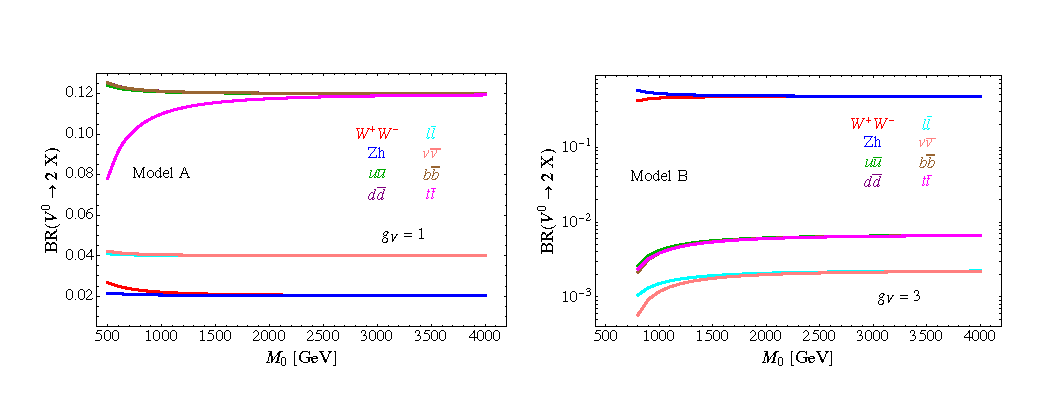
\includegraphics[width=0.99\textwidth]{figures/theory/hvtmodels.pdf}
\caption{Predicted branching fractions of a \PZpr for two explicit HVT models: Model  $\mathrm{A}_{g_V=1}$ (left) and model $\mathrm{B}_{g_V=3}$ (right)~\cite{Pappadopulo:2014qza}.}
\label{fig:theory:hvtBR}
\end{figure}

\subsubsection{Warped extra dimensions}
\label{sec:theory:wed}
Extra dimensional theories also offer solutions to the hierarchy problem. This thesis focuses on Randall-Sundrum (RS) warped extra dimensional scenarios~\cite{PhysRevLett.83.3370}. In RS models, a new curved spatial dimension $y$ is proposed, leading to a 5-dimensional space-time bounded by two (3+1)-dimensional planes, or \emph{branes}: the UV/Planck and the IR/TeV brane. The new metric now depends on the radius $r$ and the curvature $k^{-1}$ of the new extra dimension
\begin{equation}
  ds^2=e^{-2ky}\eta_{\mu\nu}dx^{\mu}dx^{\nu}+dy^2; 0 < y < \pi R
\end{equation}
Gravity is concentrated and relatively strong at the Planck brane at $y=0$, which is separated from us by the fifth dimension. Our observed four-dimensional reality and the Standard Model particles reside at the \TeV brane, at $y=\pi R$. Only gravity, transmitted through gravitons, is allowed to propagate through the warped 5D space-time (the "bulk") and is not confined to either brane. Figure~\ref{fig:theory:rs1} illustrates how the branes and the bulk are connected.
\begin{figure}[h!]
\centering
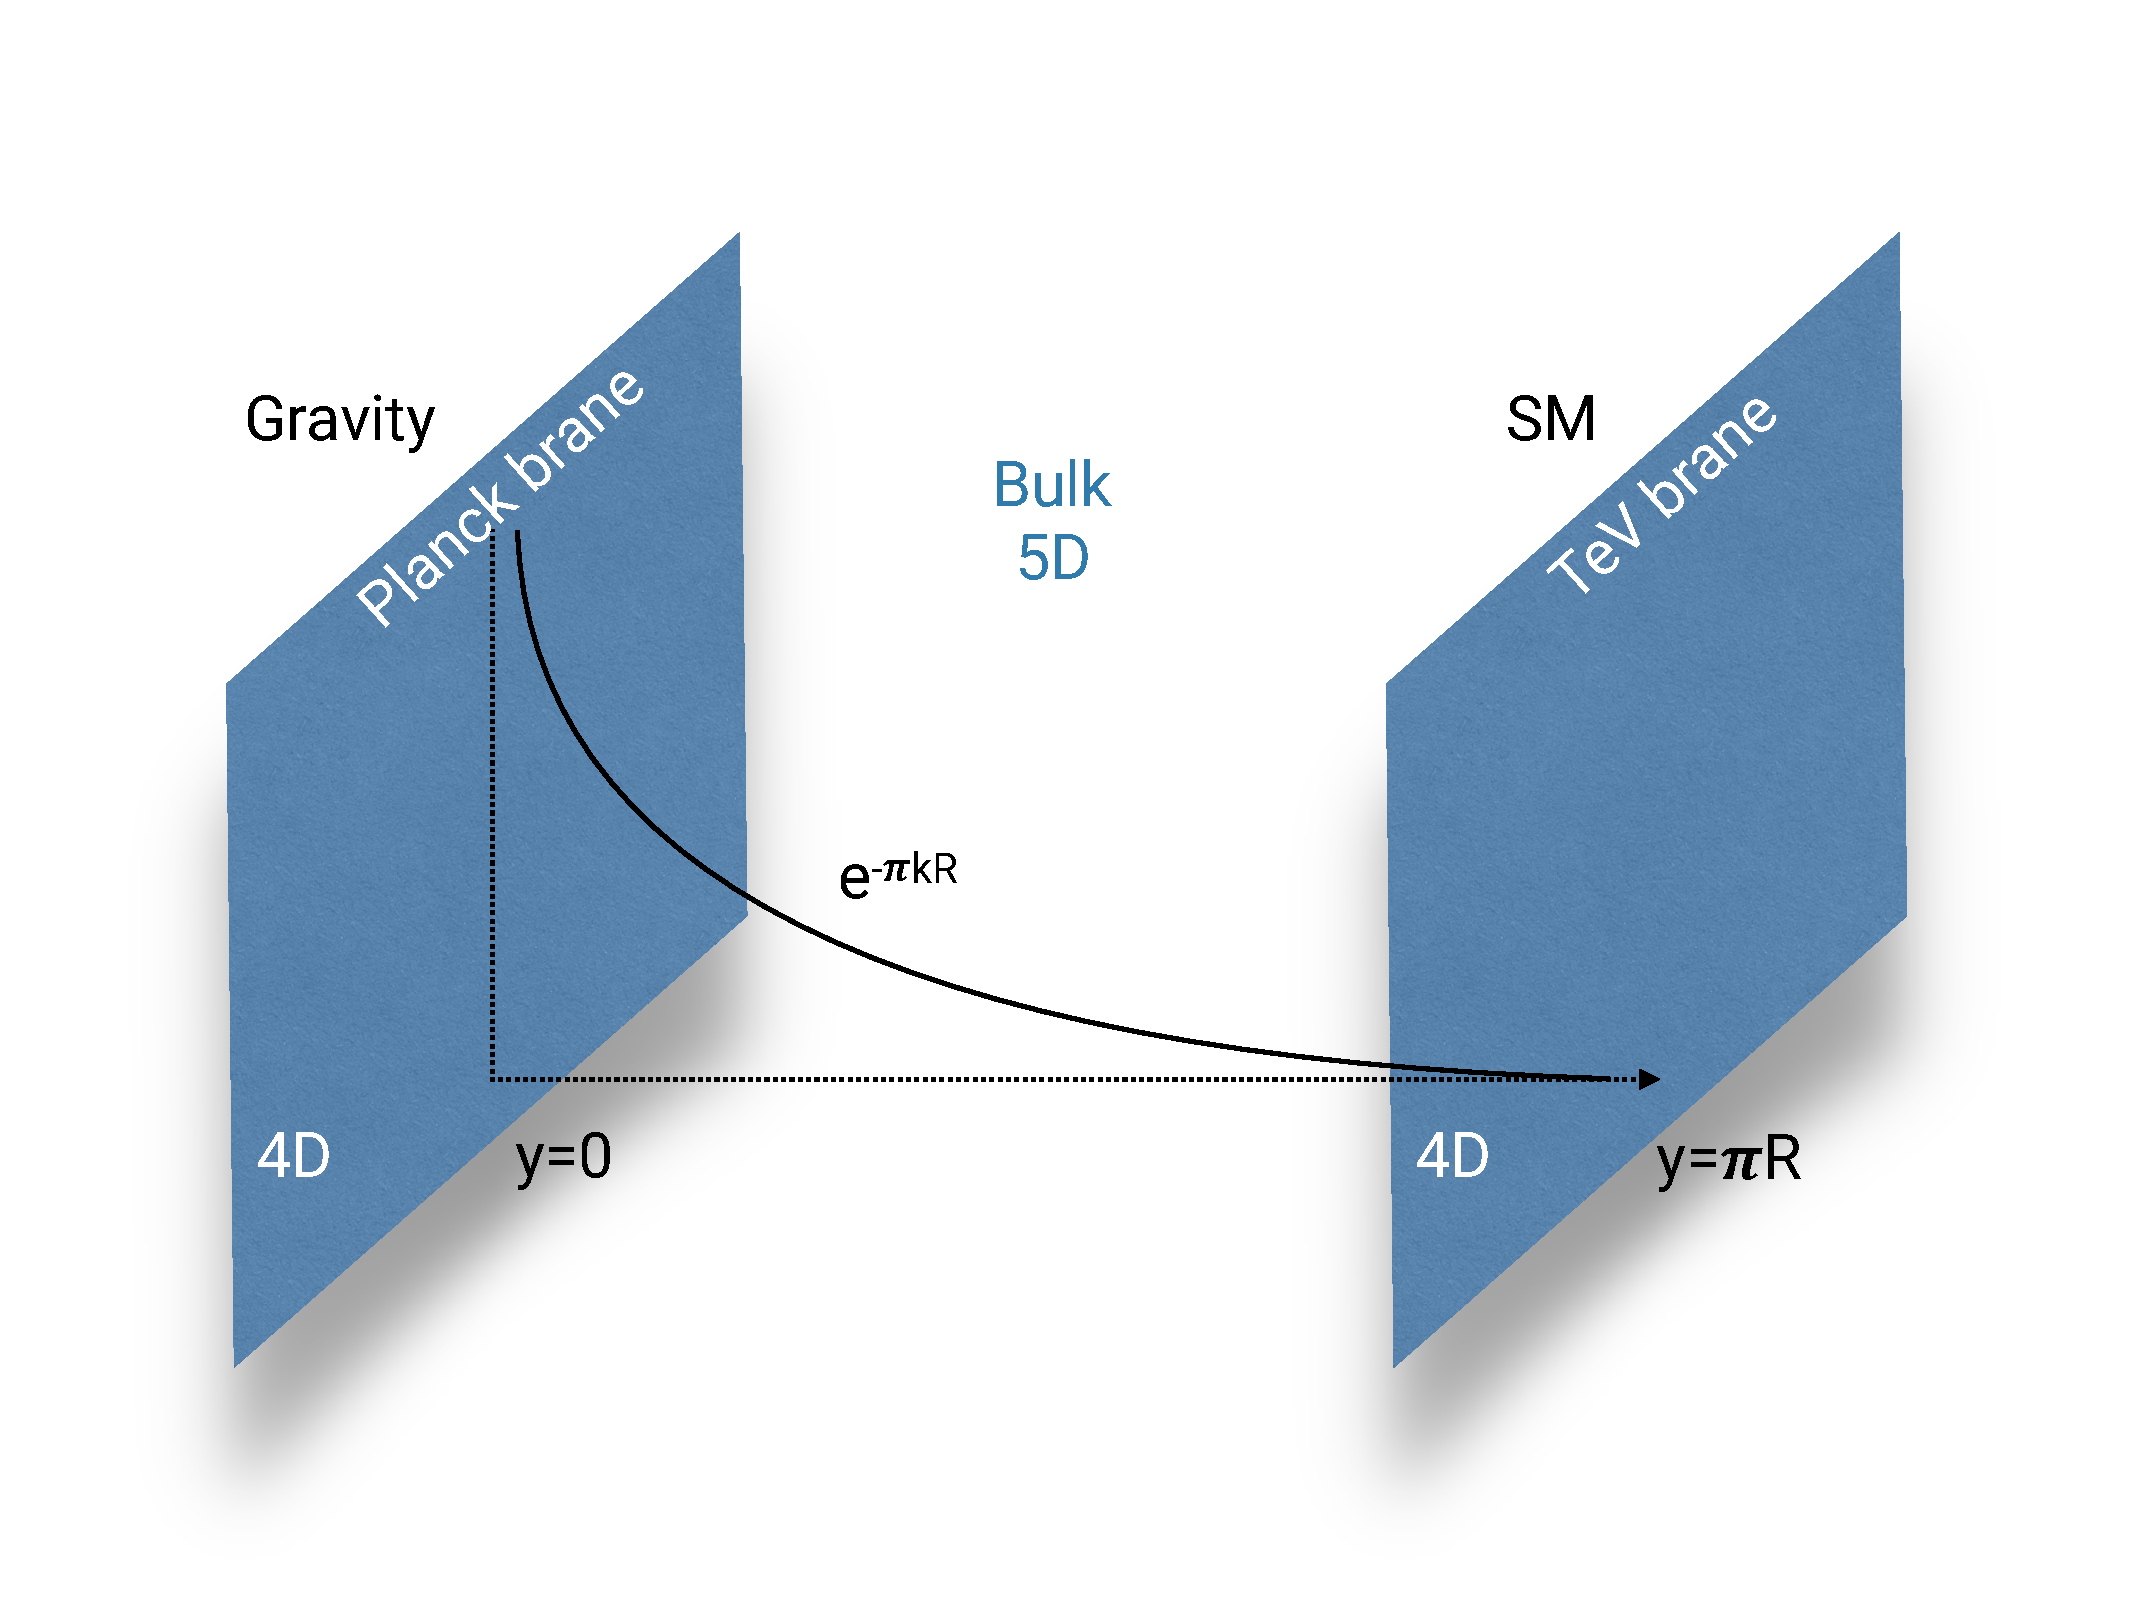
\includegraphics[width=0.49\textwidth]{figures/theory/rs1.pdf}
\caption{The RS model predicts an extra dimension where a 5D space-time stretches between two 4D branes: the Planck brane where gravity is concentrate, and the TeV brane where the SM particles are confined.}
\label{fig:theory:rs1}
\end{figure}
 Due to the warping, the Planck mass on the Planck brane gets reduced by a factor of $e^{-\pi kR}$ at the TeV brane, thereby solving the hierarchy problem. One distinct prediction of the model, and a way in which we can test its validity, is the prediction of a tower of \TeV-scale excitations with spin-2, so called Kaluza-Klein states, that could be observed in high energy experiments. \newline
In this thesis, we are more interested in an alternative to the original RS model called the "bulk" scenario~\cite{PhysRevD.76.036006,Fitzpatrick:2007qr}. In this case, the Standard Model particles, besides the Higgs boson, are also allowed to propagate in the bulk. The light 1st and 2nd generation fermions are localized near the Planck brane, yielding small couplings to the Higgs boson that still resides at the \TeV brane, explaining their small masses. Similarly, the top quark is now located near the \TeV brane, resulting in a stronger Yukawa coupling to the Higgs boson. In addition, with the gravitons located near the \TeV brane and the fermions now residing near the Planck brane, the graviton coupling to fermions is strongly suppressed. SM gluons have a flat distribution throughout the bulk, making gluon-gluon production the dominant production channel of gravitons. Due to the weak vector bosons absorbing the Higgs degree of freedom in spontaneous symmetry breaking, their wave-functions fall of steeply near the \TeV brane, resulting in a coupling to the gravitons similar to that of the Higgs and the top. The branching ratios of the Bulk Graviton is shown in Figure~\ref{fig:theory:bulk}.
\begin{figure}[h!]
\centering
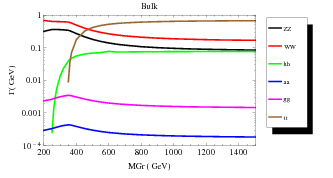
\includegraphics[width=0.49\textwidth]{figures/theory/BulkGravitonBR_tuomas.png}
\caption{Predicted branching fractions for a Bulk Graviton.}
\label{fig:theory:bulk}
\end{figure}

